%%%%%%%%%%%%%%%%%%%%%%%%%%%%%%%%%%%%%%%%%%%%%%%%%%%%%%%%%%
% # The Present Studies
%%%%%%%%%%%%%%%%%%%%%%%%%%%%%%%%%%%%%%%%%%%%%%%%%%%%%%%%%%

\chapter{The Present Studies}\label{ch-study}

% \excnt=107

This chapter introduces the experiments I conducted in the present dissertation. In Section~\ref{stu-rq}, I begin by reviewing the research questions that guided the project. Section~\ref{stu-study} explains my choice to include separate studies on ORCs and SRCs, and Sections~\ref{stu-procedure}--\ref{stu-slw} lay the groundwork for the coming chapters by detailing the sequencing of tasks, the stimulus selection procedures, and the distribution of gapped vs. resumptive RCs in the three languages of interest. Section~\ref{stu-consultant} provides information about the language consultants who helped me create the Korean and Mandarin experimental materials, Sections~\ref{stu-participant}--\ref{stu-proficiency} describe my participant samples, and Section~\ref{stu-analysis} outlines the data analysis procedures used in the experiments. Section~\ref{stu-conclusion} concludes the chapter.

%========================================================%
\section{Research questions}\label{stu-rq}
%========================================================%

This section lays out the four main research questions (RQs) that I investigate in the dissertation, most of which have theoretical implications that go beyond the narrow examination of gapped vs. resumptive RCs in L1/L2 English.

\subsection{RQ 1: Does resumption ease both production and comprehension of RCs under processing strain?}

As we saw in Chapter~\ref{ch-resumption}, it is widely acknowledged that L1 English resumption eases RC production under processing strain, but there is disagreement about whether this also holds for RC comprehension. Supporters of the selfish speaker model (\cite{ferreira.swets2005}; \cite{morgan.etal2020}; \cite{polinsky.etal2013}), for instance, claim that resumption only benefits speakers.

While there are a number of L1 adult English studies purportedly showing that resumption eases processing during RC comprehension with reference to, e.g., binary forced-choice judgment data (\cite{ackerman.etal2018}), comprehensibility judgment data (\cite{beltrama.xiang2016}), and self-paced reading data (\cite{hammerly2022}; \cite{hofmeister.norcliffe2013}), only one of them directly tested whether resumption helps with accurate RC interpretation: \textcite{hammerly2022}, who found that accuracy was equally high for gaps and RPs (p.~828ff). What is more, the study by \textcite{morgan.etal2020}---which specifically probed RC interpretation and found that RPs impede comprehension---used stimuli containing distractors (NPs that are other potential antecedents, i.e., with matching features, for the RP), and this effectively nullified any benefits that might have otherwise been conferred by resumption. Thus there is need for additional research that directly tests whether resumption helps with accurate interpretation of RCs (\cite{meltzer-asscher2021}, p.~191).

The experiments in the present dissertation address this lacuna in the research by testing for processing effects in the production and comprehension of gapped vs. resumptive RCs. To do this, I use an elicited production task (EPT) during language production and a self-paced reading task (SPRT) during language comprehension. Crucially, the SPRT contains comprehension questions whose correct answer requires accurate resolution of the RC dependency.

Regarding the latter task, more is at stake here than just the effect that resumption has on RC comprehension. For supporters of the selfish speaker model, determining whether resumption assists with comprehension has repercussions for our understanding of the relationship between the production and comprehension systems more generally. If the data point toward resumption facilitating only production and not comprehension, so the argument goes, it would indicate that there is a nontrivial rift between the two systems (\cite{ferreira.swets2005}, p.~277). If, however, the data point toward resumption being helpful for comprehension as well as for production, this would cast doubt on the notion that such a rift exists. 

\subsection{RQ 2: What is the status of resumptive RCs in English interlanguages?}

Observing that some L2ers consistently produce resumptive RCs even in syntactic environments where they are disallowed in both the L1 and the target language, \textcite{hyltenstam1984,hyltenstam1990} and \textcite{eckman2004} hypothesized that the interlanguage grammars of such L2ers license resumption in at least some domains (see~Section~\ref{acq-preliminary}). I test this hypothesis by collecting acceptability judgments from L2ers---in the target language (English) as well as in their L1 (Korean or Mandarin). If there are L2ers who consistently (i.e.,~in ≥ 80\% of trials) accept RPs even in syntactic environments where they do not accept them in the L1, this would be compatible with the view that they have grammatical resumption that cannot be directly attributed to an external source. If, however, the L2 judgment data indicate that consistent RP acceptance is generally traceable to L1 transfer, this would present a problem for the argument advanced by Hyltenstam and Eckman that L2ers default to resumption in some or all RC environments in the early stages of L2 acquisition.

\subsection{RQ 3: What is the relationship between competence and performance in L2 acquisition?}

As discussed in Section \ref{acq-assumption}, it has often been assumed in the traditional L2 literature on, \textit{inter alia}, RC resumption that L2ers' production patterns reflect representations licensed by their interlanguage grammars. This assumption, which I call the performance-competence correspondence assumption (PCCA), requires testing because it has long been acknowledged in other areas of linguistic research that performance and competence do not always go hand in hand (e.g.,~\cite{chomsky1965}, p.~4). In fact, the L1 adult literature touching on RC resumption shows that English native speakers can easily be induced into producing RCs with RPs in islands even though they consistently reject the same types of RCs in offline judgment tasks (e.g.,~\cite{ferreira.swets2005}), suggesting that they consider such RCs to be ill-formed. 

The experiments described in the following chapters put the PCCA to the test by comparing the results from the EPT to the results from an acceptability judgment task (AJT). If L2ers consistently accept resumptive RCs in the same environments where they produce them, it would indicate that they regard resumption as a licit option for relativization in those environments. If, on the other hand, L2ers consistently reject resumptive RCs in any given environment in the AJT, it would suggest that the resumptive RCs they produce in that same environment are processing resumptives rather than grammatical resumptives---just as the data indicate is the case for English native speakers (see Section \ref{res-wellformedness}).

While the idea that L2 resumptive RCs are linked to processing seems plausible enough (\cite{hyltenstam1984}, p.~55), it has not yet undergone thorough psycholinguistic testing for both production and comprehension. Also, prior to the present dissertation, there were few L2 studies investigating resumptive RCs in long-distance or island environments, despite research (e.g.,~\cite{morgan.wagers2018}) showing that deeper levels of embedding make RC processing more difficult for native speakers. I address these understudied areas by examining the processing and acceptability of gapped vs. resumptive RCs in the context of the short-distance vs. long-distance vs. \textit{wh}-island (SLW) hierarchy, drawing on methodological practices honed over the past two decades in the L1 processing literature (e.g.,~\cite{ferreira.swets2005,hammerly2022,hofmeister.norcliffe2013,morgan.etal2020,morgan.wagers2018}).

\subsection{RQ 4: If some L2ers do consistently accept RPs, can they ever become sensitive to the English prohibition on resumption in RCs?}

The dissertation also examines the manner in which restructuring occurs during L2 acquisition of RCs, as mapped out in Section \ref{acq-initial-state}. Specifically, it investigates whether restructuring is a strictly additive process or if instead new options motivated by the target language input (e.g.,~gapping at DO) can overwrite options transferred from the L1 (e.g.,~resumption at DO). If more advanced L1-Mandarin L2ers reject English RPs in RC domains where their lower-proficiency counterparts accept them, this would suggest that purging resumptive RCs from interlanguages is possible, in accordance with the overwriting approach. If it is the case, on the other hand, that even high proficiency L1-Mandarin L2ers persist in accepting RPs in English RCs, this would suggest that it is difficult if not impossible to overwrite (some) resumptive RC options transferred from the L1.

%========================================================%
\section{ORC and SRC studies}\label{stu-study}
%========================================================%

There are two studies in the present dissertation: one examining direct object RCs (ORCs) and the other examining subject RCs (SRCs). The experimental materials used in these studies differ only with respect to the critical stimuli and are otherwise identical. Each study consisted of a language background questionnaire (LBQ), an~elicited production task (EPT), a~self-paced reading task (SPRT), English/Korean/Mandarin acceptability judgment tasks (AJTs), a~C-test, and a short exit survey. The materials for each of these tasks can be found in the appendices, as laid out in Table \ref{tab:task}.

\begin{table}
\caption{Tasks included in the ORC and SRC studies}\label{tab:task}
\raggedright\setstretch{1}
\begin{tabularx}{\linewidth}{lLl}\toprule
Task & Purpose & Appendix \\\midrule
LBQ & Collect demographic information about participants & \ref{app-lbq} \\
EPT & Test whether resumption facilitates RC production & \ref{app-materials-ept} \\
SPRT & Test whether resumption facilitates RC comprehension & \ref{app-materials-spr} \\
AJTs & Test the acceptability of gapped and resumptive RCs & \ref{app-materials-ajt} \\
C-test & Assess English proficiency & \ref{app-zenker} \\
Exit survey~~ & Collect information on participants' experiences in the experiments & \ref{app-exit} \\\bottomrule
\end{tabularx}
\vspace{-12pt}
\end{table}

\noindent The participants in the two studies were also sampled from the same populations (no participants took part in both studies). Each study had a group of English native speaker controls (ENSs), a group of L1-Korean L2ers of English (KLEs), and a group of L1-Mandarin L2ers of English (MLEs).

The ORC and SRC versions of the experiments each come with certain advantages.\footnotemark{} The ORC study, for its part, is optimized for clean comparisons across conditions. As the SPRT item in Table \ref{tab:spr-condition-orc} demonstrates, the gap or RP always occurs at the same point in the sentence in the ORC version of the task---immediately following the tenth word. Furthermore, the words immediately preceding and following the gap or RP are the same across all conditions. This uniformity might explain why so many previous studies have focused exclusively on ORCs (e.g.,~\cite{beltrama.xiang2016,hammerly2022,heestand.etal2011,hofmeister.norcliffe2013}).

\footnotetext{I discuss the exact makeup of each task (critical conditions, fillers, etc.) in subsequent chapters: Chapter~\ref{ch-ept} for the ORC/SRC EPTs, Chapter~\ref{ch-spr} for the ORC/SRC SPRTs, and Chapter~\ref{ch-ajt} for the ORC/SRC AJTs.}

\begin{table}
\caption{Critical conditions in the ORC self-paced reading task}\label{tab:spr-condition-orc}
\raggedright\setstretch{1}
\begin{tabularx}{\linewidth}{lL}\toprule
Environment & Example stimulus in the gap and RP conditions \\\midrule
Short-distance~~~ & I think Mary knows the man that these detectives arrested \{\_\_/*him\} \linebreak at the beginning of the week. \\
Long-distance & Mary knows the man that I think these detectives arrested \{\_\_/*him\} \linebreak at the beginning of the week. \\
\textit{Wh}-island & Mary knows the man that I wonder which detectives arrested \{*\_\_/*him\} \linebreak at the beginning of the week. \\\bottomrule
\end{tabularx}
\vspace{-12pt}
\end{table}

An example SPRT item from the SRC study is shown in Table \ref{tab:spr-condition-src} for comparison. While these stimuli still allow for clean comparisons between gapping trials and resumption trials within each level of the \textsc{environment} factor, they make for rather messier comparisons across levels of \textsc{environment} than in the ORC study. Notice that the position of the gap/RP in the sentence and the words immediately surrounding the gap/RP both vary across conditions due to (a)~the variable placement of the \textit{think}-clause in the short-distance vs. long-distance conditions and (b)~the fronting of the \textit{wh}-phrase in the \textit{wh}-island condition.

\begin{table}
\caption{Critical conditions in the SRC self-paced reading task}\label{tab:spr-condition-src}
\raggedright\setstretch{1}
\begin{tabularx}{\linewidth}{lL}\toprule
Environment & Example stimulus in the gap and RP conditions \\\midrule
Short-distance~~~ & I think Mary knows the man that \{\_\_/*he\} borrowed this book \linebreak at the beginning of the month. \\
Long-distance & Mary knows the man that I think \{\_\_/*he\} borrowed this book \linebreak at the beginning of the month. \\
\textit{Wh}-island & Mary knows the man that I wonder which book \{*\_\_/*he\} borrowed \linebreak at the beginning of the month. \\\bottomrule
\end{tabularx}
\vspace{-12pt}
\end{table}

What makes the SRC study useful is that it maximizes the contrast in processing difficulty across conditions. On the assumption that single-clause SRCs are easier to process than single-clause ORCs (e.g.,~\cite{just.etal1996,king.just1991,lau.tanaka2021,traxler.etal2002}), the SRC study's [Gap, Short] condition should be the easiest one to process in the entire project (see~Section~\ref{gap-so}). By contrast, because island effects are thought to be stronger in SRCs than in ORCs (e.g.,~\cite{han.etal2012,keffala.goodall2011,morgan.wagers2018}), the SRC study's [Gap, Island] condition should be the hardest one to process in the entire project (see~Section~\ref{gap-wi}). 

Another reason to include an SRC study is that, as mentioned in Section \ref{res-wellformedness}, there is some evidence that L1-English adults may resort to resumption more often in SRCs than in ORCs. Suggestively, perhaps, the 174 L1-English resumption tokens in my informally-collected corpus (https://osf.io/xwgfz) contained more SRCs (75/174~= 43\%) than ORCs (55/174~= 32\%); see also Chapter~\ref{ch-resumption}, fn.~2. By comparison, the 41 L2-English resumption tokens were more or less evenly distributed between ORCs (18/41~= 44\%) and SRCs (16/41~= 39\%).\footnotemark{}

\footnotetext{The L1s of these L2ers included but were not limited to Arabic, Hebrew, Korean, Mandarin, Persian, and Spanish.}

%========================================================%
\section{Procedure}\label{stu-procedure}
%========================================================%

The main tasks for each study were the EPT, the SPRT, and the English/Korean/Mandarin AJTs. Each participant also completed a consent form, an LBQ, the English proficiency C-test, and a short exit survey (see~Table~\ref{tab:task}); all testing occurred asynchronously over the internet. The tasks were administered in the following order: consent form $\rightarrow$ LBQ $\rightarrow$ EPT $\rightarrow$ SPRT $\rightarrow$ English AJT $\rightarrow$ Korean/Mandarin AJT (L2ers only) $\rightarrow$ C-test $\rightarrow$ exit survey. ENSs completed all the tasks in a single experimental session, whereas for KLEs and MLEs the tasks were distributed across five shorter sessions (Session~1: consent form, LBQ, EPT; Session~2: SPRT; Session~3: English AJT; Session~4: Korean/Mandarin AJT; Session~5: C-test, exit survey). At the end of each session, L2ers received a password to access the next one. They could proceed to the following session immediately or save it for later, as long as they finished all five sessions within seven days of starting. 

My reasons for having the tasks in this order are as follows: The EPT was administered before the other main tasks so that participants would not be primed to produce certain types of RCs based on stimuli they had seen in the other tasks. Because the AJT, in which participants were asked to rate sentences for acceptability, was the task that ran the greatest risk of putting participants in a metalinguistic frame of mind, it was placed after the other two main tasks (the EPT and the SPRT) so as to minimize the chance that participants would use explicit morphosyntactic knowledge during those tasks. L2ers took the English version of the AJT before the version in their L1 to minimize L1-to-L2 influence in their acceptability judgments. Finally, the C-test was given after the main tasks to limit fatigue earlier in the experiment, since previous experience had indicated that L2ers find these sorts of fill-in-the-blank tasks particularly taxing.

A progress bar was provided at the top of the screen during all tasks involving multiple trials; it was hidden during the instructions and reset to zero at the beginning of each new task. During pilot testing,\footnotemark{} I found that adding this progress bar led to a sharp reduction in remarks/complaints about the length of the experiments. The median time that it took each group was as follows: in the ORC study, 59 minutes for ENSs, 83 minutes for KLEs, 119 minutes for MLEs; in the SRC study, 57 minutes for ENSs, 93 minutes for KLEs, and 122 minutes for MLEs.

\footnotetext{There were multiple rounds of pilot testing focusing on different tasks and involving different versions of the stimuli. In the largest single round of pilot testing, 33~ENSs and 33~KLEs completed earlier versions of the EPT and the English/Korean AJTs (see~\cite{zenker.schwartz2022}).}

For each task, as mentioned above, the ORC and SRC versions differed only in terms of the critical stimuli. The EPT, SPRT, and AJT stimuli were Latin-squared such that participants saw each item in a given task in only one condition. Participants also received different running lists for the SPRT, the English AJT, and (for L2ers) the Korean/Mandarin AJT---all of which had very similar stimuli---to ensure that they would not encounter any one item more than once in the same condition across tasks. In addition, the stimuli were pseudorandomized so that critical items never appeared in consecutive trials; the exact sequencing of stimuli was determined by an algorithm and therefore varied across participants. The experiments were built using the jsPsych library (\cite{deleeuw2015}) and hosted on Cognition (\url{https://www.cognition.run}). The credits for the images used in the experiments are provided in Appendix \ref{app-image}.

%========================================================%
\section{Selection of lexical items for the stimuli}\label{stu-stimuli}
%========================================================%

The lexical items used in the stimuli for the EPT, the SPRT, and the AJTs were drawn from the official list of 2,315 basic English vocabulary words used by the Korean Ministry of Education, Science, and Technology (MEST, \citeyear{ministryofeducationscienceandtechnology2008}) and from the top 5,000 lemmas in the Corpus of Contemporary American English (\cite{davies2010}). Words needed to appear on at least one of these lists to be considered for inclusion in the critical and filler stimuli; this was done to maximize the likelihood that L2ers would be familiar with all the lexical items used in the tasks.

Special care was required when it came to selecting the verbs governing the gap/RP in each critical sentence for the ORC study. For one thing, in experimental studies concerned with the processing of direct object filler-gap dependencies, it is important to use strongly transitive verbs because doing so encourages participants to posit a gap (\cite{omaki.schulz2011}). Because experimental stimuli needed to be converted into Korean and Mandarin for the L1 AJTs, the verbs also needed to have translation equivalents in Korean and Mandarin that are both (a) one word in length and (b) capable of taking a direct object. Verbs for which the Korean and/or Mandarin analog instead takes a dative object or prepositional phrase were excluded. It was also necessary to consider whether each verb would yield natural-sounding control sentences across all three languages in the study.

Following discussion with my Korean and Mandarin language consultants (see~Section~\ref{stu-consultant} below), I~selected 15 verbs for inclusion in the ORC study stimuli: \textit{arrest}, \textit{catch}, \textit{defend}, \textit{employ}, \textit{examine}, \textit{fire}, \textit{hire}, \textit{interview}, \textit{punish}, \textit{question}, \textit{recruit}, \textit{release}, \textit{rescue}, \textit{treat}, and \textit{welcome}. To confirm that these verbs were strongly transitive, I conducted a corpus analysis on the 14.5-million-word Open American National Corpus (OANC; \url{https://anc.org}). For good measure, the transitivity bias of the 15 verbs selected for the SRC study were also checked via the same procedure. The details of these analyses can be found in Appendix~\ref{app-transitivity}, and the results are shown in Tables~\ref{tab:transitivity-orc} and \ref{tab:transitivity-src}. All verbs had transitivity rates in excess of 80\%, indicating that they are strongly transitive and therefore appropriate for use in the stimuli. With the exception of \textit{interview} and \textit{fire}, all the ORC study verbs ranked in the top 50\% of verbs in the corpus for transitivity bias.

\begin{table}
\caption{Transitivity rates for verbs in the ORC study}\label{tab:transitivity-orc}
\raggedright\setstretch{1}
\begin{tabularx}{\linewidth}{XYYYY}\toprule
Verb & Transitive Tokens & Total Tokens & Transitivity Rate & Percent Rank\\\midrule
\csvreader[late after line=\\,late after last line=\\\bottomrule]
{../analysis/tables/orc_trans_automated.csv}{}{\csvcoli & \csvcolii & \csvcoliii & \csvcoliv & \csvcolv}
\end{tabularx}
\textit{Note}. Verbs organized by transitivity rate.
\vspace{-12pt}
\end{table}

\begin{table}
\caption{Transitivity rates for verbs in the SRC study}\label{tab:transitivity-src}
\raggedright\setstretch{1}
\begin{tabularx}{\linewidth}{XYYYY}\toprule
Verb & Transitive Tokens & Total Tokens & Transitivity Rate & Percent Rank\\\midrule
\csvreader[late after line=\\,late after last line=\\\bottomrule]
{../analysis/tables/src_trans_automated.csv}{}{\csvcoli & \csvcolii & \csvcoliii & \csvcoliv & \csvcolv}
\end{tabularx}
\textit{Note}. Verbs organized by transitivity rate.
\vspace{-12pt}
\end{table}

%========================================================%
\section{Well-formedness of gapped and resumptive RCs in the SLW hierarchy}\label{stu-slw}
%========================================================%

As discussed in Section \ref{acq-slw}, the present dissertation expands on previous L2 research by examining a set of processing asymmetries for RCs that I refer to as the short-distance vs. long-distance vs. \textit{wh}-island (henceforth, SLW) hierarchy. My expectations regarding the well-formedness of gapped and resumptive RCs in the relevant environments for the three language of interest are shown in Table \ref{tab:slw}.

\begin{table}
\caption{Distribution of gapping (−), resumption (+), and unrelativizable domains (0) in the SLW hierarchy}\label{tab:slw}
\raggedright\setstretch{1}
\begin{tabularx}{\linewidth}{llXXX}\toprule
Study & Language & Short-distance & Long-distance & \textit{Wh}-island \\\midrule
ORC~~~~ & English & − & − & 0 \\
ORC & Korean & − & − & N/A \\
ORC & Mandarin~~~~~~~~~~ & ± & ± & N/A \\
SRC & English & − & − & 0 \\
SRC & Korean & − & − & N/A \\
SRC & Mandarin & − & ± & N/A \\\bottomrule
\end{tabularx}
\textit{Note}. `N/A' indicates that the level is irrelevant because the language lacks that RC environment.
\vspace{-12pt}
\end{table}

Based on the judgments of my language consultants (see Section \ref{acq-slw-pathway}), I expected that L1 speakers of English, Korean, and Mandarin would all allow gapping in both short-distance and long-distance RCs and that Mandarin speakers would additionally allow resumption in long-distance RCs (for both ORCs and SRCs) and short-distance ORCs (but not short-distance SRCs). I also expected L1-English speakers not to allow either gapping or resumption in \textit{wh}-island RCs. Finally, since it is impossible in Korean and Mandarin (with their head-final RCs) to replicate the situation where a filler needs to be reactivated in an embedded question introduced by another filler (a~moved \textit{wh}-phrase), I treat the \textit{wh}-island level as not applicable (N/A) in those languages (see~Sections~\ref{gap-lw} and \ref{acq-slw-pathway}). I therefore expected that English \textit{wh}-island RCs translated into Korean and Mandarin would be functionally equivalent to regular long-distance RCs.

With regard to processing difficulty in English RCs, I expected that none of the groups would have much trouble in the short-distance condition, especially in the SRC study. For ENSs, I expected that the long-distance condition would be only slightly more difficult than the short-distance condition. It is important to note that the types of sentences I used in the long-distance condition, as in (\ref{ex-complexity-a}), were much less complex than those used in L1 adult (English) studies like \textcite{hofmeister.norcliffe2013}, as in (\ref{ex-complexity-b}). 

\pex\label{ex-complexity}
\a Long-distance SPRT stimulus in the ORC study of this dissertation: \par\nobreak\vspace{5pt}\label{ex-complexity-a}
Mary knows the man that I think these detectives arrested \{\_\_/*him\} at the beginning \linebreak of the week.
\a Long-distance SPRT stimulus in Hofmeister and Norcliffe's study: \par\nobreak\vspace{5pt}\label{ex-complexity-b}
Mary confirmed that there was a prisoner who the prison officials had acknowledged that the guard helped \{\_\_/*him\} to make a daring escape. \par\nobreak\vspace{5pt}
\hfill (adapted from \cite{hofmeister.norcliffe2013}, p. 229, (6a) and (6b))
\xe 

\noindent For L2ers, however, I expected that the long-distance condition would cause more difficulty than for ENSs on the assumption that processing in general requires more effort in a nonnative language than in an L1 (\cite{hopp2014,kilborn1992}). Processing difficulty, after all, is not an absolute notion: What is easy for native speakers may be difficult for L2ers, and what is easy for advanced L2ers may be difficult for intermediate L2ers. I deliberately made the long-distance environment less strenuous than in L1 adult processing research so as to highlight these sorts of differences in processing efficiency based on L1 background and L2 proficiency. Finally, I~expected that all groups would show signs of processing difficulty in the \textit{wh}-island condition due to the high processing cost associated with extending a filler-gap dependency into an embedded question introduced by a moved \textit{wh}-phrase, especially with such RCs being (a)~ill-formed in English and (b)~rarely if ever encountered in the English input.

%========================================================%
\section{Language consultants}\label{stu-consultant}
%========================================================%

While developing the sentence templates I would use for the critical conditions in the Korean and Mandarin AJTs, I solicited feedback from 14 language consultants in total: seven native speakers of Korean and seven native speakers of Mandarin. Most of these consultants were current or former students at the University of Hawai`i at Mānoa in the Department of East Asian Languages and Literatures, the Department of Linguistics, or the Department of Second Language Studies. For each language, I worked closely with one of these consultants to draft up the final list of stimuli and instructions (which were close translations of the stimuli and instructions in the English AJT), and an additional consultant read and gave feedback on the completed materials before data collection commenced. The consultant who helped me most with the Korean materials grew up in Incheon, Korea, and the one who helped me most with the Mandarin materials grew up in Taipei, Taiwan. The Korean materials were presented in Hangul script and the Mandarin materials were presented in traditional Chinese characters.

%========================================================%
\section{Participants}\label{stu-participant}
%========================================================%

The participant samples for the ORC and SRC studies consisted of ENSs, KLEs, and MLEs. ENSs were recruited on Prolific (\url{https://www.prolific.com}) and through the Linguistics Beyond the Classroom (LBC) program at the University of Hawai`i at Mānoa (\url{http://ling.lll.hawaii.edu/sites/lbc}). KLEs were recruited on Korean university websites such as SNULife (\url{https://www.snulife.com}) and Ewhaian (\url{http://www.ewhaian.com}) as well as on Korean job boards such as Spec Up (\url{https://cafe.naver.com/specup}). MLEs were recruited exclusively on Taiwan's PTT Bulletin Board System (\url{https://www.ptt.cc}).\footnotemark{} Participants gave informed consent before starting the experiment and were compensated with either course credit (LBC participants only) or a small monetary award.

\footnotetext{hence the use of traditional Chinese characters in the Mandarin version of the AJT}

Participants needed to be 18 years of age or older to participate. For ENSs, the only other requirements were that they (a) were native speakers of English and (b) grew up in the United States. To qualify for participation, KLEs and MLEs needed to (a) have an English age of onset (AO) of eight years or older (see~below) and (b) be native speakers of Korean or Mandarin, respectively.

To ensure that the KLEs and MLEs were genuine L2ers of English, I required that they each have an English AO of eight years or older. Previous experimental work on L1 acquisition has found that children tend to reach adultlike competence for most complex morphosyntactic phenomena between the ages of three and six (e.g.,~\cite{aravind.etal2018}; \cite{crain.thornton2012}; \cite{kazanina.phillips2001}). If KLEs and MLEs who start learning English at age eight or later already have a more or less fully-formed L1 grammar in place at the point that they start acquiring English, we can be confident that they are \textit{bona fide} L2ers of English (and certainly not simultaneous bilinguals). In addition, some L2 studies have presented evidence that developing targetlike knowledge of morphosyntactic properties starts to become both less successful and less uniform with an AO around age seven, if not earlier (e.g.,~\cite{granena.long2013}, p.~326; \cite{hyltenstam1992}, p.~364; \cite{johnson.newport1989}, p.~79; see~also \cite{sadeghi2022}, p.~134), further reinforcing the idea that adult speakers who started learning a language at age eight or older are distinct from L1 adults.

Power analyses performed on L1/L2 pilot study data using the \textit{simr} package (\cite{green.macleod2016}) in R (\cite{rcoreteam2023}) indicated that at least 60 participants per group would be needed to achieve sufficient power (≥~80\%) for detecting a significant processing effect for resumption in the reading time data from the SPRT. The SPRT was the most power-hungry of the tasks owing to the small effect sizes typically obtained in reading time analyses (\cite{avery.marsden2019}). My minimum recruiting target was therefore 60 participants per group for the final round of data collection. 

The participants' self-reported demographic data from the LBQ are presented in aggregate form in Table \ref{tab:participants}. A handful of Prolific participants were excluded because I judged them not to be L1 speakers of American English based on their audio recordings for the EPT (sometimes in conjunction with other evidence, such as IP addresses); those participants are not included in the table.

\begin{table}
\caption{Participant background information prior to data cleaning}\label{tab:participants}
\raggedright\setstretch{1}
\begin{tabularx}{\linewidth}{XXrrrrrrrrrrr}\toprule
\multicolumn{4}{c}{} & \multicolumn{3}{c}{Age at Testing} & \multicolumn{3}{c}{Age of Onset} & \multicolumn{3}{c}{Years in Anglosphere}\\\cmidrule(lr){5-7}\cmidrule(lr){8-10}\cmidrule(l){11-13}
Study & Group & $n$ & \%~Female & Mean & \textit{SD} & Range & Mean & \textit{SD} & Range & Mean & \textit{SD} & Range\\\midrule
\csvreader[late after line=\\,late after last line=\\\bottomrule]
{../analysis/tables/participants.csv}{}{\csvcoli & \csvcolii & \csvcoliii & \csvcoliv & \csvcolv & \csvcolvi & \csvcolvii & \csvcolviii & \csvcolix & \csvcolx & \csvcolxi & \csvcolxii & \csvcolxiii}
\end{tabularx}
\vspace{-12pt}
\end{table}

\noindent The L2 groups were roughly matched in terms of age at testing, English AO, and years of residence in English-speaking countries. Because age has traditionally been measured differently in Korea than in Taiwan and the United States (\cite{mccurry2022}), KLEs were asked to give their age in terms of years from date of birth. Nearly all KLEs and MLEs were living in their home countries (Korea and Taiwan, respectively) at the time of testing (KLE-ORC: 67/69~= 97\%; KLE-SRC: 65/66~= 98\%; MLE-ORC: 75/76~= 99\%; MLE-SRC: 73/73~= 100\%). 

%========================================================%
\section{Experience learning other languages}\label{stu-language}
%========================================================%

The LBQ included questions asking participants about their experience learning different languages, as shown in (\ref{stu-ex-question}).

\pex Questions asked about each language in the LBQ \label{stu-ex-question}
\a Name of language
\a Proficiency level (Beginner, Low Intermediate, High Intermediate, Advanced, Near-Native, Native)
\a Age when you started learning this language (From Birth, 1, 2, 3, etc.)
\a Did your primary caregivers speak this language to you when you were a child?
\a Percentage of total weekly listening/speaking/reading/writing time spent using this language
\a Number of years spent studying this language as a second or foreign language (if~applicable)
\xe 

\noindent It should come as no surprise that many of the participants had been exposed to other languages besides those in my experiments (for ENSs: English; for KLEs: English and Korean; for MLEs: English and Mandarin). In total, 28\% of participants in the ORC study (ENS: 44\%; KLE: 29\%; MLE: 8\%) and 19\% of participants in the SRC study (ENS: 25\%; KLE: 29\%; MLE: 5\%) reported that they had spent at least some time learning another language. Tables~\ref{tab:stu-lang-orc-ens}--\ref{tab:stu-lang-src-mle} give an overview of participants' learning history for these other languages. 

\begin{table}
\caption{Exposure to other languages among ENSs in the ORC study (sorted by participant counts)}\label{tab:stu-lang-orc-ens}
\raggedright\setstretch{1}
\begin{tblr}{colspec = {X[l]rrrrr}} 
\toprule 
Language & $n$ & ~~~~~~AO Mean & ~~~~~~AO Range & ~~~~~~Self-Rating Mean & ~~~~~~Self-Rating Range \\ 
\midrule 
Spanish & 17 & 14.71 & 0--62 & 2.41 & 1--6\\
Japanese & 9 & 17.44 & 10--33 & 2.22 & 1--3\\
French & 7 & 16.29 & 12--21 & 2.00 & 1--3\\
Korean & 5 & 24.40 & 17--50 & 1.80 & 1--3\\
Mandarin & 4 & 10.00 & 0--20 & 2.00 & 1--3\\
German & 3 & 15.33 & 13--17 & 1.67 & 1--2\\
ASL & 1 & 17.00 & N/A & 3.00 & N/A\\
Hawaiian & 1 & 15.00 & N/A & 2.00 & N/A\\
Tagalog & 1 & 18.00 & N/A & 1.00 & N/A\\
Thai & 1 & 15.00 & N/A & 3.00 & N/A\\
\bottomrule
\end{tblr}\newline
\textit{Note}. AO~= age of onset; self-ratings ranged from 1~(beginner) to 6~(native).
\vspace{-12pt}
\end{table}

\begin{table}
\caption{Exposure to other languages among KLEs in the ORC study (sorted by participant counts)}\label{tab:stu-lang-orc-kle}
\raggedright\setstretch{1}
\begin{tblr}{colspec = {X[l]rrrrr}} 
\toprule 
Language & $n$ & ~~~~~~AO Mean & ~~~~~~AO Range & ~~~~~~Self-Rating Mean & ~~~~~~Self-Rating Range \\ 
\midrule 
French & 7 & 16.00 & 10--19 & 1.71 & 1--2\\
Mandarin & 6 & 16.17 & 13--19 & 1.67 & 1--3\\
Japanese & 4 & 10.50 & 0--16 & 2.00 & 1--3\\
Spanish & 3 & 20.33 & 17--22 & 1.33 & 1--2\\
German & 1 & 23.00 & N/A & 1.00 & N/A\\
Indonesian & 1 & 36.00 & N/A & 3.00 & N/A\\
Vietnamese & 1 & 30.00 & N/A & 1.00 & N/A\\
\bottomrule
\end{tblr}\newline
\textit{Note}. AO~= age of onset; self-ratings ranged from 1~(beginner) to 6~(native).
\vspace{-12pt}
\end{table}

\begin{table}
\caption{Exposure to other languages among MLEs in the ORC study (sorted by participant counts)}\label{tab:stu-lang-orc-mle}
\raggedright\setstretch{1}
\begin{tblr}{colspec = {X[l]rrrrr}} 
\toprule 
Language & $n$ & ~~~~~~AO Mean & ~~~~~~AO Range & ~~~~~~Self-Rating Mean & ~~~~~~Self-Rating Range \\ 
\midrule 
Japanese & 3 & 19.67 & 17--22 & 1.33 & 1--2\\
Hokkien & 2 & 0.00 & N/A & 4.50 & 3--6\\
Spanish & 2 & 18.00 & N/A & 1.50 & 1--2\\
French & 1 & 18.00 & N/A & 3.00 & N/A\\
German & 1 & XX & N/A & 2.00 & N/A\\
Italian & 1 & XX & N/A & 1.00 & N/A\\
Korean & 1 & 37.00 & N/A & 1.00 & N/A\\
Russian & 1 & XX & N/A & 1.00 & N/A\\
Thai & 1 & XX & N/A & 1.00 & N/A\\
\bottomrule
\end{tblr}\newline
\textit{Note}. AO~= age of onset; XX~= no data; self-ratings ranged from 1~(beginner) to 6~(native).
\vspace{-12pt}
\end{table}

\begin{table}
\caption{Exposure to other languages among ENSs in the SRC study (sorted by participant counts)}\label{tab:stu-lang-src-ens}
\raggedright\setstretch{1}
\begin{tblr}{colspec = {X[l]rrrrr}} 
\toprule 
Language & $n$ & ~~~~~~AO Mean & ~~~~~~AO Range & ~~~~~~Self-Rating Mean & ~~~~~~Self-Rating Range \\ 
\midrule 
Spanish & 10 & 11.00 & 0--22 & 2.40 & 1--5\\
ASL & 2 & 17.00 & 15--19 & 1.50 & 1--2\\
French & 2 & 12.50 & 11--14 & 2.50 & 2--3\\
German & 2 & 15.50 & 13--18 & 1.00 & 1--1\\
Italian & 1 & 7.00 & N/A & 2.00 & N/A\\
\bottomrule
\end{tblr}\newline
\textit{Note}. AO~= age of onset; self-ratings ranged from 1~(beginner) to 6~(native).
\vspace{-12pt}
\end{table}

\begin{table}
\caption{Exposure to other languages among KLEs in the SRC study (sorted by participant counts)}\label{tab:stu-lang-src-kle}
\raggedright\setstretch{1}
\begin{tblr}{colspec = {X[l]rrrrr}} 
\toprule 
Language & $n$ & ~~~~~~AO Mean & ~~~~~~AO Range & ~~~~~~Self-Rating Mean & ~~~~~~Self-Rating Range \\ 
\midrule 
Japanese & 8 & 17.00 & 9--24 & 2.50 & 1--4\\
Mandarin & 6 & 16.17 & 13--18 & 1.67 & 1--3\\
German & 5 & 20.80 & 16--26 & 1.20 & 1--2\\
French & 1 & 18.00 & N/A & 1.00 & N/A\\
Spanish & 1 & 19.00 & N/A & 3.00 & N/A\\
\bottomrule
\end{tblr}\newline
\textit{Note}. AO~= age of onset; self-ratings ranged from 1~(beginner) to 6~(native).
\vspace{-12pt}
\end{table}

\begin{table}
\caption{Exposure to other languages among MLEs in the SRC study (sorted by participant counts)}\label{tab:stu-lang-src-mle}
\raggedright\setstretch{1}
\begin{tblr}{colspec = {X[l]rrrrr}} 
\toprule 
Language & $n$ & ~~~~~~AO Mean & ~~~~~~AO Range & ~~~~~~Self-Rating Mean & ~~~~~~Self-Rating Range \\ 
\midrule 
Korean & 2 & 20.50 & 18--23 & 2.00 & 1--3\\
Hokkien & 1 & 6.00 & N/A & 4.00 & N/A\\
Japanese & 1 & 18.00 & N/A & 1.00 & N/A\\
\bottomrule
\end{tblr}\newline
\textit{Note}. AO~= age of onset; self-ratings ranged from 1~(beginner) to 6~(native).
\vspace{-12pt}
\end{table}

One ENS in the ORC study reported that she was also a native speaker of Spanish, and five additional ENSs (four in the ORC study and one in the SRC study) indicated that they were heritage speakers of another language (Mandarin:~2; Spanish:~2; Tagalog:~1).\footnotemark{} The one ENS who was a potential heritage speaker of Tagalog gave seemingly contradictory responses: While she reported that her primary caregivers spoke Tagalog to her when she was a child, she also reported that she did not start learning the language until she was 18 (see~Table~\ref{tab:stu-lang-orc-ens}).

\footnotetext{For present purposes, I define a heritage language speaker as anyone who answered the question ``Did your primary caregivers speak this language to you when you were a child?'' in the affirmative while also indicating that s/he was not a native speaker of that language.}

Only one KLE reported that she had started learning a language other than English or Korean prior to age 9; this participant, who took part in the ORC study, indicated that she had started learning Japanese from birth. This may have been an error, though, because she also reported that (a)~her level of Japanese proficiency was only 1 out of 6, (b)~none of her caregivers spoke Japanese to her when she was a child, and (c)~she had spent only a year learning Japanese.

The MLE participants were not specifically asked about their experience with other varieties of Chinese, but three individuals self-identified as speakers of Hokkien: one was an MLE in the ORC study who reported that she was a native speaker of both Hokkien and Mandarin, the second was an MLE in the ORC study who reported that her proficiency level in Hokkien was 3 out of 6, and the third was an MLE in the SRC study who reported that she was a heritage speaker of Hokkien with a self-assessed proficiency level of 4 out of 6. Although Mandarin replaced Hokkien as the dominant variety of Chinese spoken in Taiwan in the mid-20th century (\cite{chiung2017}, p.~39), Hokkien remains widely spoken there, and it is reasonable to assume that most of my MLE participants have some degree of familiarity with the language. (One of my Mandarin language consultants, who grew up in Taiwan and speaks Hokkien fluently, informed me that her ratings for the sentence types I used in the Mandarin AJT would be the same in Hokkien.) No MLEs reported that they had started to learn a language other than English, Hokkien, or Mandarin before age 17.

%========================================================%
\section{English Proficiency}\label{stu-proficiency}
%========================================================%

English proficiency was measured using a C-test of my own making. The task itself is provided in Appendix \ref{app-zenker}, and the procedure I followed for checking its reliability and validity is described in Appendix \ref{app-validation}. Two ENSs in the ORC study (2/90~= 2\%) and two MLEs in the SRC study (2/73~= 3\%) were lost from the C-test dataset due to experimental error. The C-test scores, out of a maximum of 50, for the remaining participants are plotted in Figure \ref{fig:ctest}.

\begin{figure}
\caption{English C-test proficiency scores in the ORC and SRC studies (Max~= 50)} \label{fig:ctest}
\raggedright\setstretch{1}
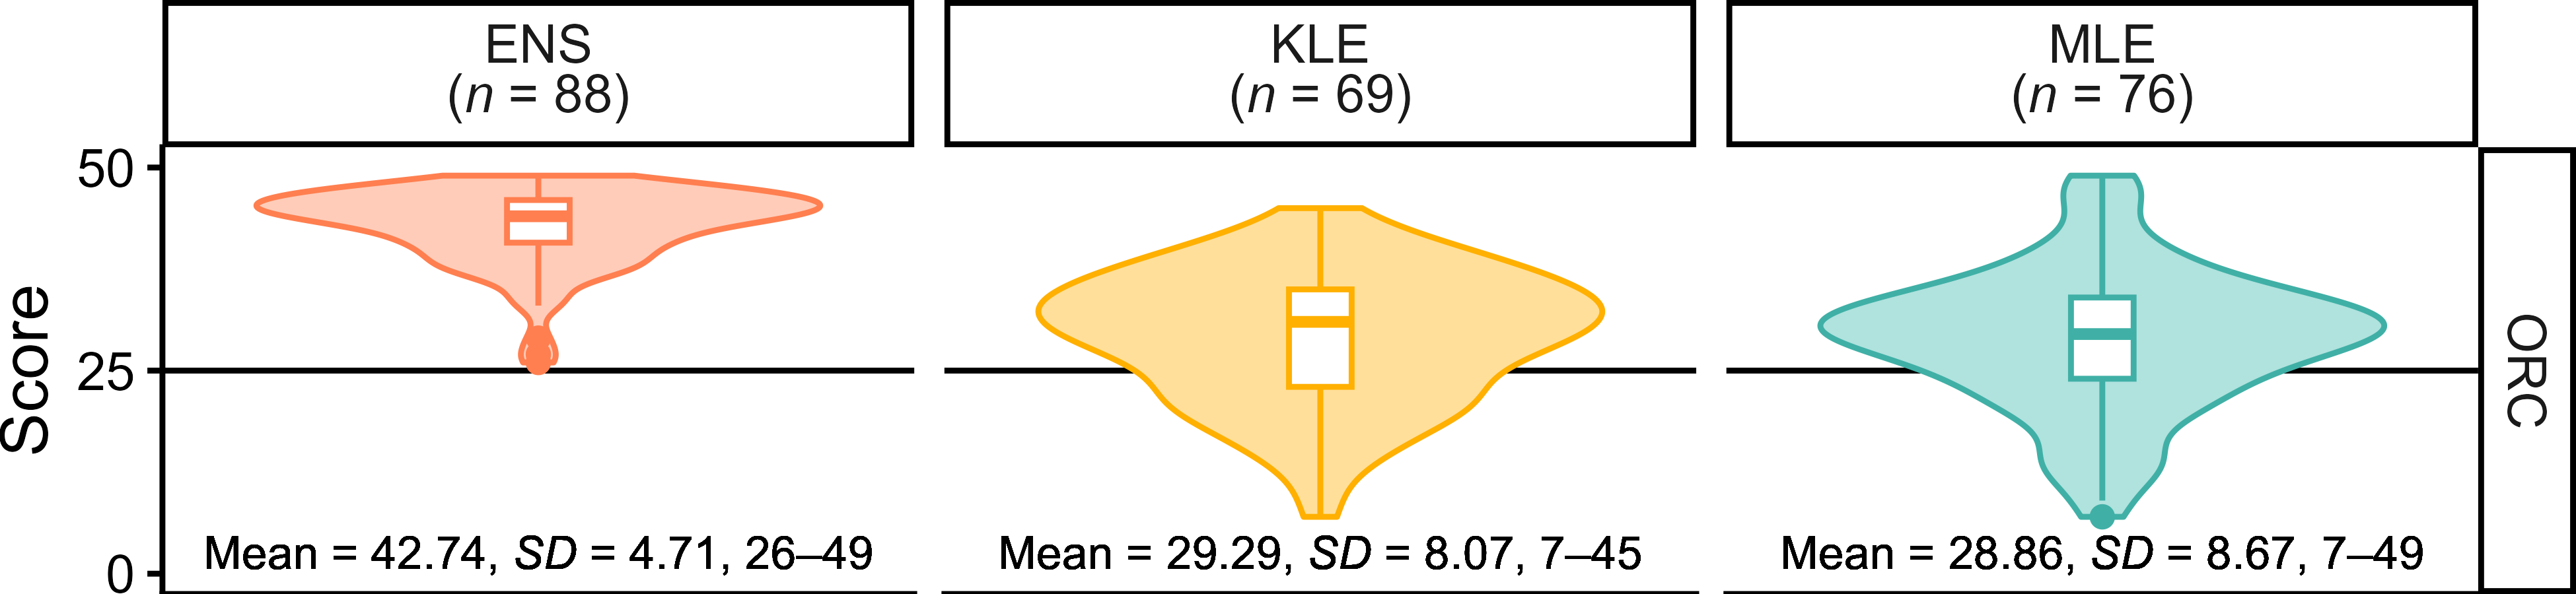
\includegraphics{../analysis/plots/orc_ctest.png}
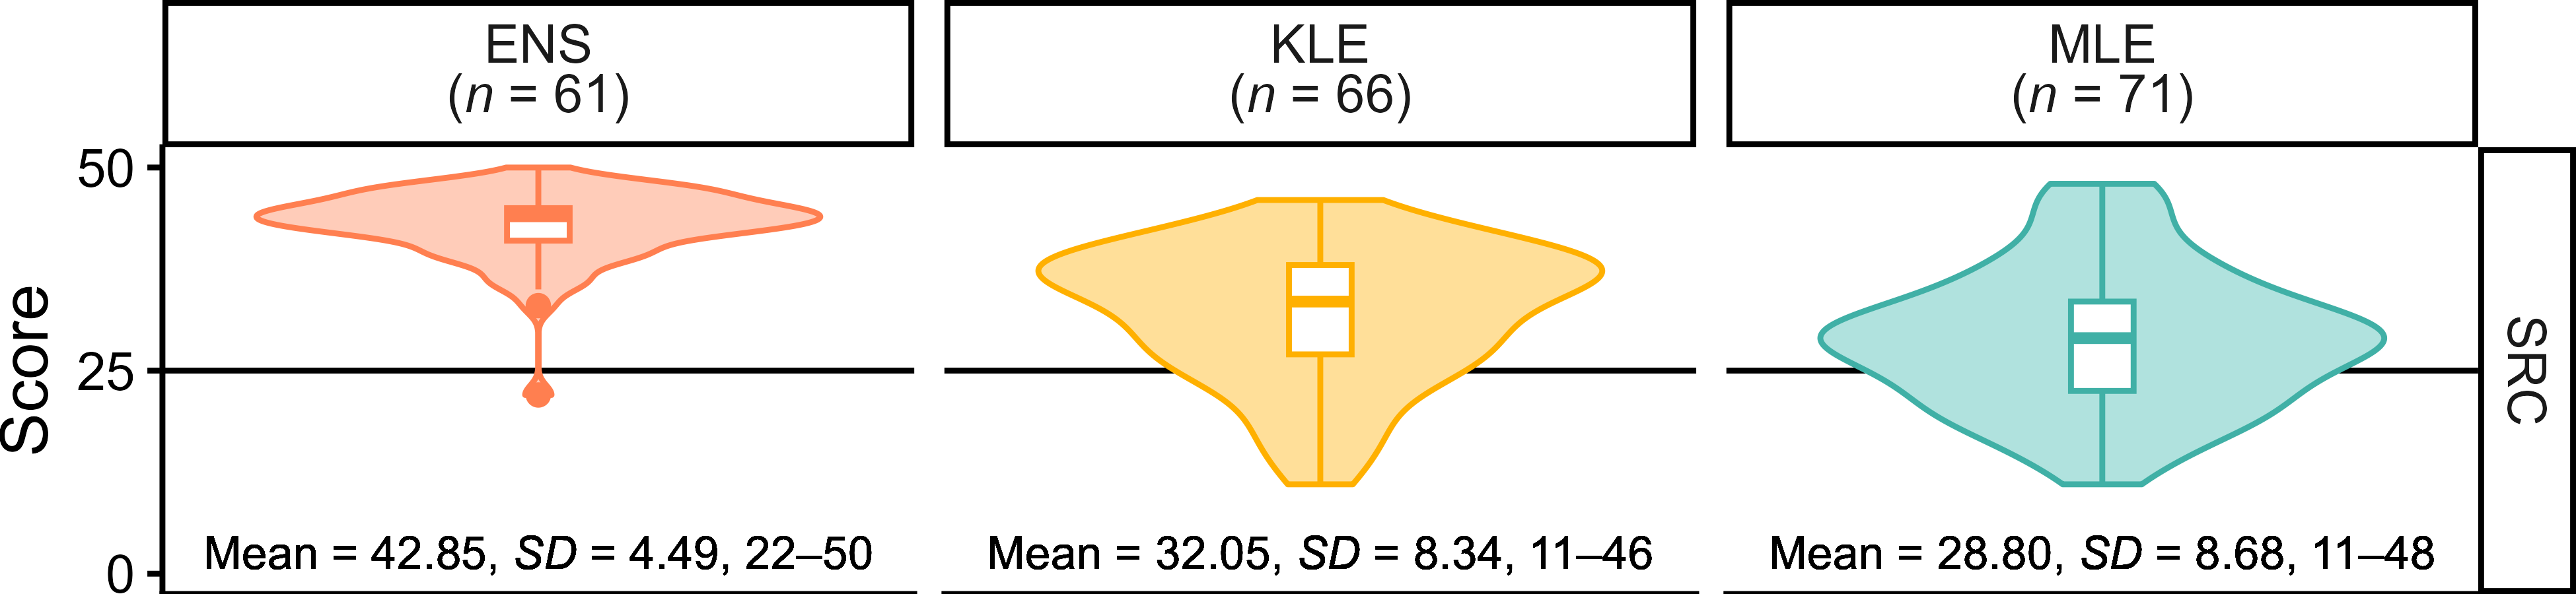
\includegraphics{../analysis/plots/src_ctest.png}
\textit{Note}. Horizontal line represents 50\% accuracy; center lines in boxplots are medians, boxes are interquartile ranges, and whiskers extend to data points within 1.5 times the interquartile range.
\vspace{-12pt}
\end{figure}

The ENS group's scores tended to be very high, as expected for native speakers of the language. The scores for KLEs and MLEs, though partially overlapping with the ENS group's scores, were much more widely dispersed, with a fair number having less than 50\% accuracy (KLE-ORC: 19/69~= 28\%; MLE-ORC: 20/76~= 26\%; KLE-SRC: 13/66~= 20\%; MLE-SRC: 21/71~= 30\%). KLEs scored slightly higher on average than MLEs did (KLE-ORC mean~= 29.29; MLE-ORC mean~= 28.86; KLE-SRC mean~= 32.05; MLE-SRC mean~= 28.80), although the range of scores was almost identical across the KLE and MLE groups for each study (KLE-ORC: 7--45; MLE-ORC: 7--49; KLE-SRC: 11--46; MLE-SRC: 11--48). Overall, these results suggest that the L2ers ranged from intermediate to advanced English proficiency.

The binary accuracy data from the C-test were examined further for each study separately using a mixed-effects logistic regression model (model formula: \textsc{accuracy \~{} group + (1~|~participant) + (1 + group | item)}---see Appendix~\ref{app-results-ctest}, Table~\ref{tab:app-orc-ctest-accuracy-model} for details). Results from the primary analysis for the ORC study showed that C-test accuracy was significantly higher for ENSs than for KLEs ($\hat{\beta}$~=~−2.45, \textit{SE}~= 0.29, $p$~<~.001) and MLEs ($\hat{\beta}$~=~−2.51, \textit{SE}~= 0.29, $p$~<~.001). Pairwise comparisons did not find a significant difference in mean accuracy scores between the KLE group and the MLE group ($p$~= .956).

The same pattern of C-test results was found for the SRC study (see Appendix~\ref{app-results-ctest}, Table~\ref{tab:app-src-ctest-accuracy-model} for details): The model yielded a significant effect for \textsc{group}, with ENSs scoring higher than both KLEs ($\hat{\beta}$~=~−2.13, \textit{SE}~= 0.31, $p$~<~.001) and MLEs ($\hat{\beta}$~=~−2.50, \textit{SE}~= 0.33, $p$~<~.001). The KLE group's scores were not found to be significantly higher than the MLE group's scores in the pairwise comparisons ($p$~= .153).

%========================================================%
\section{Data analysis}\label{stu-analysis}
%========================================================%

Data analysis and visualization were done in R (\cite{rcoreteam2023}), with the \textit{lme4} (\cite{bates.etal2015}), \textit{ordinal} (\cite{christensen2019}), and \textit{glmmTMB} (\cite{brooks.etal2017}) packages used for mixed-effects modeling. The alpha level (i.e., significance threshold) was set at .05 for all the primary analyses. Accordingly, $p$-values of .05 and smaller were treated as significant and $p$-values between .05 and .10 were treated as marginally significant. 

Categorical predictors were given simple coding to allow for canonical ANOVA-style interpretations of main effects and interactions (see~\cite{barr2021}). In simple coding, sometimes referred to as contrast coding or deviation coding, each level of a factor is compared to the reference level, with the intercept being the grand mean. Thus, the presence of a main effect for a given factor indicates that observations at the target level of the factor differ significantly from observations at the reference level, ignoring all other factors in the analysis. When numerical predictors (e.g.,~English proficiency scores from the C-test) were added to a model, they were centered and scaled via a $z$-score transformation to facilitate regression computations. Each mixed-effects model also had random effects for \textsc{participant} and \textsc{item}. Models were kept as close as possible to the maximal random-effects structure justified by the design (see~\cite{barr2021}; \cite{barr.etal2013}) while avoiding (a)~convergence errors, (b)~cases where the variance was estimated at zero for one or more of the random effects terms, and (c)~cases were one or more of the correlations between random effect terms was estimated at ±1. In these situations, the random-effects structure was simplified until the problem was resolved.

Post-hoc testing was performed using the \textit{emmeans} package (\cite{lenth2022}), with the alpha level adjusted for multiple comparisons via the multivariate $t$ distribution. In line with the \textit{emmeans} package's default settings, the Kenward-Roger method (\cite{kenward.roger1997}) was used to calculate degrees of freedom and adjust covariance matrices for post-hoc tests unless the number of observations exceeded 3,000, in which case the asymptotic method was used instead to reduce computation time.

Many of the mixed-effects models in this dissertation have complex structures such that it would be inconvenient to report the full fixed-effects output in the main text, especially since it is often the post-hoc tests rather than the full-model analyses that are of primary interest. For this reason, the results tables are placed in the appendices and cross-referenced in the main text.

%========================================================%
\section{Summing up}\label{stu-conclusion}
%========================================================%

Marking the commencement of the experimental portion of the dissertation, this chapter started by reviewing the main research questions that motivated this project and proceeded to provide information about the construction and administration of the tasks, the participants recruited to take part in the experiments, and the procedures employed for data analysis. The next three chapters are organized by task, with the ORC results presented alongside the SRC results. We begin in the next chapter with the elicited production task.